\section{Elaboración del circuito impreso}

En la figura \ref{fig:pcb-implementada} se puede observar la placa impresa ya perforada,
previo a la soldadura de los componentes.
Se comprobó que todos los componente elegidos en el software tuvieran la misma distribución de pines que en su versión física. 
Se imprimió una primera versión y se realizaron correcciones en base a los resultados obtenidos al probar los componentes. \cite{pcb-atei}

\begin{figure}[H]
    \centering
    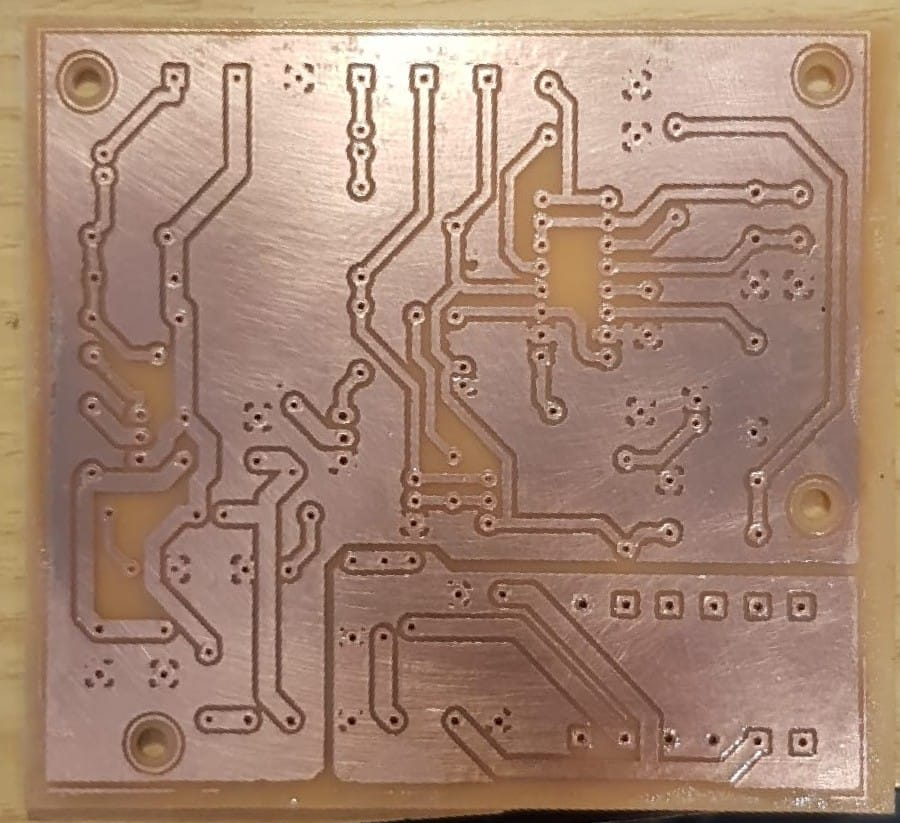
\includegraphics[width=0.8\textwidth]{images/pcb-implementada.jpeg}
    \caption{Placa impresa previo a la soldadura.}
    \label{fig:pcb-implementada}
\end{figure}

A continuación, se detallan todos los criterios aplicados para la inclusión de cada componente en el circuito impreso en base a las recomendaciones 
proporcionadas por la cátedra, los integrantes del ATEI y las especificadas en las hojas de datos de los circuitos integrados.

\paragraph{Orificios}

Los orificios se hicieron de $0.8mm$, independiente del componente. En caso de necesitar uno más grande se lo ensanchó con mecha.
Por ejemplo, para jumpers, potenciómetros y conectores macho el orificio es de $1mm$. 

\paragraph{Pads}

Con forma circular para facilitar la soldadura, excepto para la red de tierra con pads cuadrados.
Su tamaño es de $2mm$ de diámetro para los circulares y $2mm$ de lado para los cuadrados.
En los casos donde las pistas están muy cerca de los pads y no fue posible reubicarlas,
se modificó la forma o el tamaño del pad para cumplir con la distancia especificada entre pistas.  

\paragraph{Pistas}

Dado que para corrientes más altas se necesitan pistas más anchas, las pistas de potencia son lo más cortas, directas y gruesas posibles mediante la siguiente regla:
pistas finas de $1mm$ y pistas gruesas de $2mm$. 
La separación entre las pistas y el plano de tierra o cualquier otra pista es de $0.7mm$. 
Se evitó que las pistas tengan ángulos de $90^{\circ}$. 
Si en el planchado se trabaja con una temperatura excesiva las pistas se ensanchan, por lo tanto,
para evitar contactos entre pines, las pistas ingresan a los circuitos integrados de forma paralela. 

\paragraph{Tierra} 

Con el fin de mantener la aislación provista por el transformador de potencia, 
el plano de tierra se dividió en dos: una parte para el lado primario y la otra para su secundario.

\paragraph{Tornillos}

En cada extremo de la placa se realizaron orificios para los tornillos de $6mm$ de diámetro (medida de la cabeza de tornillo típica). 

\paragraph{Puntos de prueba}

Se colocaron puntos se prueba para poder medir tensiones en distintos puntos de la placa.

\paragraph{Medición de corriente} 

Se colocaron jumpers en serie con cada componente o lugar
en el que se desea medir corriente para contrastar con los resultados obtenidos por simulación.
Posteriormente los mismos fueron reemplazados por cables
para poder utilizar las puntas de corriente del osciloscopio.
